%% Direttive TeXworks:
% !TeX root = ../../presentazione.tex
% !TEX encoding = UTF-8 Unicode
% !TEX program = arara
% !TEX TS-program = arara
% !TeX spellcheck = it-IT

\section{L'interfaccia implementata}\label{sec:new}

\begin{frame}
    \frametitle{\insertsection}
    \centering
    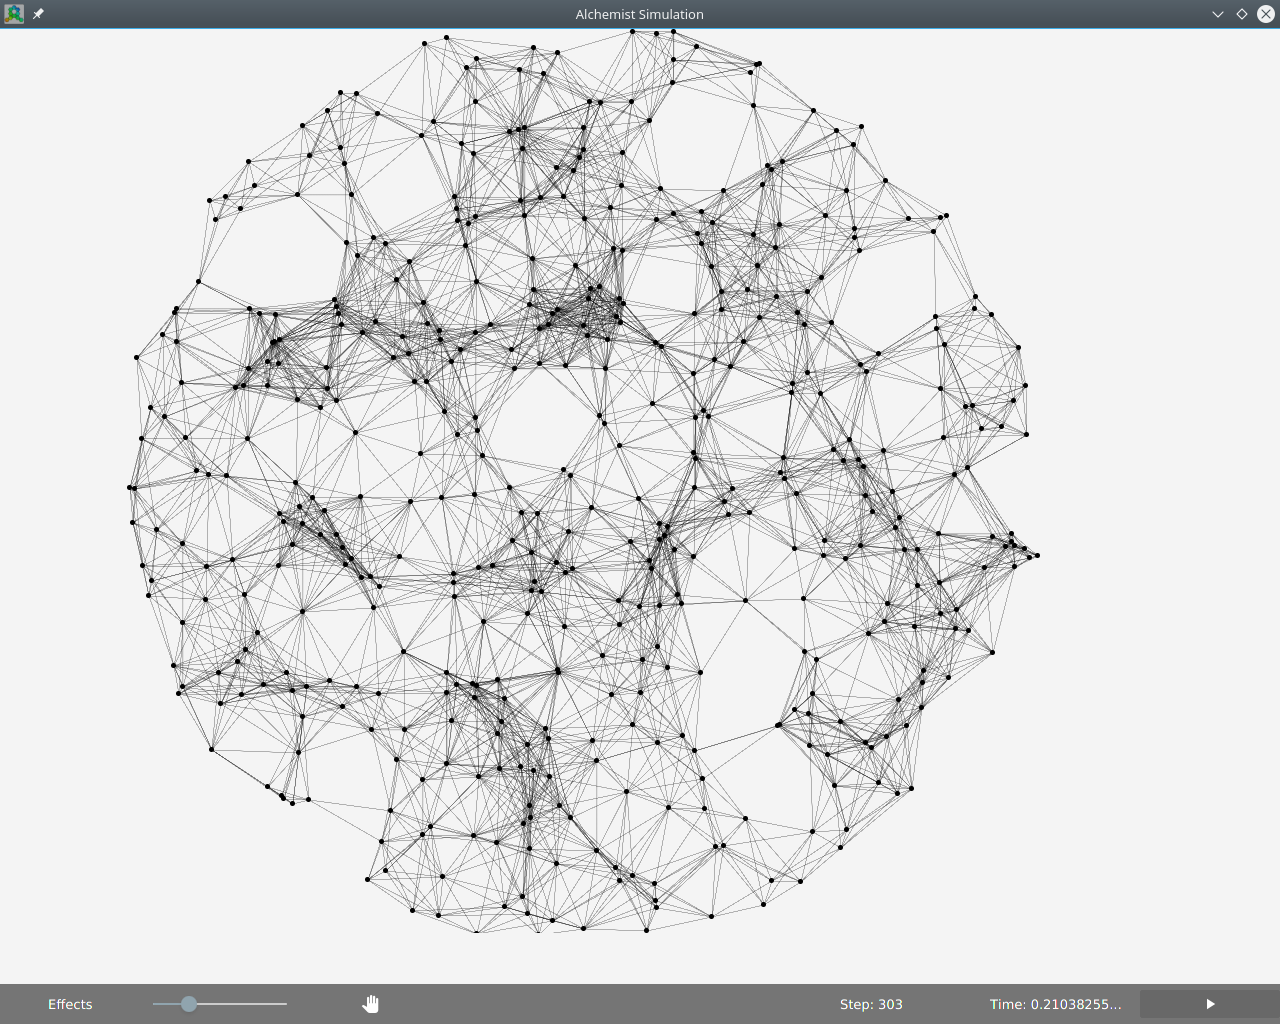
\includegraphics[scale=0.27]{img/new/window_all}
\end{frame}

\subsection{Caratteristiche}\label{subsec:feature}
\begin{frame}
    \frametitle{\insertsection}
    \framesubtitle{\insertsubsection}
    \begin{itemize}[<+(1)->]
        \item
            La libreria utilizzata per la nuova interfaccia è JavaFX.
        \item
            L'ambiente di simulazione è stato rinnovato ed è in grado di renderizzare correttamente gli effetti applicati per una simulazione.
            Inoltre, l'utente è in grado di visualizzare in tempo reale l'avanzamento della simulazione in termini di tempo e step tramite contatori dedicati.

        \item
            La gestione degli effetti risulta immediata all'utilizzo, con bottoni dedicati al salvataggio e al caricamento dei file JSON che aprono l'interfaccia fornita dal \engEmph{file manager} del sistema operativo per la scelta del file.

            È possibile modificare l'ordine di effetti e gruppi di effetti nella pila con un semplice \engEmph{drag'n'drop}.
    \end{itemize}
\end{frame}

\begin{frame}
    \frametitle{\insertsection}
    \framesubtitle{\insertsubsection}
    \begin{itemize}[<+(1)->]
        \item
            Sono stati realizzati effetti standard per la rappresentazione di nodi e collegamenti, che possono essere utilizzati da altri sviluppatori come punto di partenza per realizzare rappresentazioni più complesse e flessibili.

        \item
            L'interfaccia non utilizza valori di misura assoluti e scala senza problemi su diversi tipi di risoluzione e densità di pixel.

        \item
            È possibile controllarne il flusso di esecuzione sia tramite la pressione del tasto ``play/pausa'' che attraverso una scorciatoia da tastiera ed è possibile effettuare uno zoom nell'ambiente rappresentato eseguendo uno scroll.
    \end{itemize}
\end{frame}

\subsection{Prestazioni}\label{subsec:benchmark}
\begin{frame}
    \frametitle{\insertsection}
    \framesubtitle{\insertsubsection}
    \centering
    \begin{tabular}{ccccc}
        \multicolumn{2}{c}{\textbf{Con render}} &  & \multicolumn{2}{c}{\textbf{Senza render}} \\
         &  &  &  &  \\ \cline{1-2} \cline{4-5}
        \multicolumn{2}{|c|}{\textbf{Nuova GUI}} & \multicolumn{1}{c|}{} & \multicolumn{2}{c|}{\textbf{Nuova GUI}} \\ \cline{1-2} \cline{4-5}
        \multicolumn{1}{|c|}{Nodi + Link:} & \multicolumn{1}{c|}{$1,3153ms$} & \multicolumn{1}{c|}{} & \multicolumn{1}{c|}{Nodi + Link:} & \multicolumn{1}{c|}{1,2648ms} \\ \cline{1-2} \cline{4-5}
        \multicolumn{1}{|c|}{Solo Nodi:} & \multicolumn{1}{c|}{$0,3041ms$} & \multicolumn{1}{c|}{} & \multicolumn{1}{c|}{Solo Nodi:} & \multicolumn{1}{c|}{$0,2855ms$} \\ \cline{1-2} \cline{4-5}
         &  &  &  &  \\ \cline{1-2} \cline{4-5}
        \multicolumn{2}{|c|}{\textbf{Vecchia GUI}} & \multicolumn{1}{c|}{} & \multicolumn{2}{c|}{\textbf{Vecchia GUI}} \\ \cline{1-2} \cline{4-5}
        \multicolumn{1}{|c|}{Nodi + Link:} & \multicolumn{1}{c|}{$1,1059ms$} & \multicolumn{1}{c|}{} & \multicolumn{1}{c|}{Nodi + Link:} & \multicolumn{1}{c|}{$0,6584ms$} \\ \cline{1-2} \cline{4-5}
        \multicolumn{1}{|c|}{Solo Nodi:} & \multicolumn{1}{c|}{$0,6841ms$} & \multicolumn{1}{c|}{} & \multicolumn{1}{c|}{Solo Nodi:} & \multicolumn{1}{c|}{$0,6696ms$} \\ \cline{1-2} \cline{4-5}
    \end{tabular}
\end{frame}
